\documentclass[12pt,letterpaper]{article}
\usepackage{fullpage}
\usepackage{float}
\usepackage[top=2cm, bottom=4.5cm, left=2.5cm, right=2.5cm]{geometry}
\usepackage{amsmath,amsthm,amsfonts,amssymb,amscd}
\usepackage{lastpage}
\usepackage{enumerate}
\usepackage{fancyhdr}
\usepackage{mathrsfs}
\usepackage{xcolor}
\usepackage{graphicx}
\usepackage{listings}
\usepackage{hyperref}
\usepackage[spanish]{babel}

\hypersetup{%
  colorlinks=true,
  linkcolor=blue,
  linkbordercolor={0 0 1}
}
 \newcommand\scalemath[2]{\scalebox{#1}{\mbox{\ensuremath{\displaystyle #2}}}}
\renewcommand\lstlistingname{Algorithm}
\renewcommand\lstlistlistingname{Algorithms}
\def\lstlistingautorefname{Alg.}

\lstdefinestyle{Python}{
    language        = Python,
    frame           = lines, 
    basicstyle      = \footnotesize,
    keywordstyle    = \color{blue},
    stringstyle     = \color{green},
    commentstyle    = \color{red}\ttfamily
}

\setlength{\parindent}{0.0in}
\setlength{\parskip}{0.05in}

% Edit these as appropriate
\newcommand\course{C\'omputo Cient\'ifico en Probabilidad y Estad\'istica}
\newcommand\hwnumber{2}                     % <-- homework number
\newcommand\name{Francisco Valente Castro}  % <-- person name

\pagestyle{fancyplain}
\headheight 35pt
\lhead{\name}
\chead{\textbf{\Large Tarea \hwnumber}}
\rhead{\scriptsize{\course} \\ \normalsize{\today}}
\lfoot{}
\cfoot{}
\rfoot{\small\thepage}
\headsep 1.5em

\begin{document}

\section*{Problema 1}

\textbf{Implementar el algoritmo de \textit{Gram-Schmidt} modificado 8.1 del Trefet-hen (p. 58) para generar la descomposici\'on \textit{QR}}.\\

A continuaci\'on un extracto de la implementaci\'on en python.

\lstset{caption={Modified Gram-Schmidt (Trefethen pag. 58 ). De \textbf{factorization.py} . }}
\lstset{label={lst:alg1}}
\begin{lstlisting}[style = Python]
for idx in range(0, n):
    # Normalize ortogonal vector
    R[idx, idx] = np.sqrt(Q[:, idx].dot(Q[:, idx]))
    Q[:, idx] /= R[idx, idx]

    # Substract projection to q_i ortonormal vector
    for jdx in range(idx + 1, n):
        R[idx, jdx] = Q[:, idx].dot(Q[:, jdx])
        Q[:, jdx] -= R[idx, jdx] * Q[:, idx]
\end{lstlisting}



\section*{Problema 2}

\textbf{Implementar el algoritmo que calcula el estimador de m\'inimos cuadrados en una regresi\'on usando la descomposici\'on \textit{QR}.}\\

Para ajustar un polinomio de grado $p - 1$ con una regresi\'on consideramos un sistema de ecuaciones sobredeterminado, con $n > p$, de la forma : 
\begin{equation}
\mathbf {X} \boldsymbol {\beta} = \mathbf {y}  
\end{equation}

donde \textbf{X} es la matrix de Vandermonde :

\begin{equation}
\mathbf {X}=\begin{bmatrix}
1 & x_1 & x_1^2 & \dots & x_1^{p-1}\\
1 & x_2 & x_2^2 & \dots & x_2^{p-1}\\
1 & x_3 & x_3^2 & \dots & x_3^{p-1}\\
\vdots & \vdots & \vdots & \ddots &\vdots \\
1 & x_n & x_n^2 & \dots & x_n^{p-1}
\end{bmatrix},
%
\qquad \boldsymbol \beta = \begin{bmatrix}
\beta_1 \\ \beta_2 \\ \vdots \\ \beta_p \end{bmatrix},
%
\qquad \mathbf y = \begin{bmatrix}
y_1 \\ y_2 \\ \vdots \\ y_n
\end{bmatrix}
%
\end{equation}

Como el sistema es sobredeterminado, no existe una soluci\'on exacta. As\'i que formulamos un problema de \textit{M\'inimos Cuadrados} que consiste en encontrar una soluci\'on aproximada resolviendo el siguiente problema de minimizaci\'on :

\begin{equation}
\hat{\boldsymbol{\beta}} = \underset{\boldsymbol{\beta}}{\operatorname{arg\,min}}\,\bigl\|\mathbf y - \mathbf X \boldsymbol \beta \bigr\|^2
\end{equation}

La soluci\'on al problema de minimizaci\'on se calcula de manera anal\'itica derivando la expresi\'on anterior respecto a $\beta$ . De modo que la soluci\'on es, como tambi\'en vimos en clase,
\begin{equation}
(\mathbf X^{\rm T} \mathbf X )\hat{\boldsymbol{\beta}}= \mathbf X^{\rm T} \mathbf y
\end{equation}

Encontrando la factorizaci\'on \textbf{QR} de la matriz $\mathbf {X}$ podemos sustituir en la soluci\'on anterior. Obtenemos que, usando que la matriz $\mathbf{Q}$ es ortonormal,

\begin{equation}
((\mathbf Q \mathbf R )^{\rm T} (\mathbf Q \mathbf R ) )\hat{\boldsymbol{\beta}} = 
( \mathbf R ^{\rm T} \mathbf Q^{\rm T} \mathbf Q \mathbf R  )\hat{\boldsymbol{\beta}} =
( \mathbf R ^{\rm T} \mathbf R  )\hat{\boldsymbol{\beta}} =
( \mathbf R ^{\rm T} \mathbf Q ^{\rm T} ) \mathbf y
\end{equation}

Y suponiendo que la matriz $\mathbf R ^{\rm T}$ tiene inversa, obtenemos el sistema lineal ,
\begin{equation}
\mathbf R \hat{\boldsymbol{\beta}} = \mathbf Q ^{\rm T} \mathbf y
\end{equation}
que se puede resolver con el algoritmo de \textbf{Backward Substitution} puesto que $\mathbf R$ es una matriz triangular superior. De modo que podemos implementar la soluci\'on en python de la siguiente manera :

\lstset{caption={Estimador de m\'imos cuadrados. De \textbf{least\_squares.py} .}}
\lstset{label={lst:alg3}}
\begin{lstlisting}[style = Python]
def least_squares_estimator(X, Y):
    # Get QR decomposition of data matrix
    (Q, R) = qr_factorization(X)

    # Transform y vector
    Y_prime = Q.T @ Y.T

    # Solve system R * beta = y_prime
    beta = backward_substitution(R, Y_prime.T)

    return beta
\end{lstlisting}

\section*{Problema 3}

\textbf{Generar $Y$ compuesto de $y_i = sen(x_i) + \epsilon_i$ donde $\epsilon_i ~ N(0,\sigma)$ con $sigma = 0.11$ para $x_i = \frac{4 \pi i}{n}$ para $i=1,...,n$.} \textbf{Hacer un ajuste de m\'inimos cuadrados a $Y$, con descomposici\'on \textit{QR}, ajustando un polinomio de grado $p - 1$.} \\

Consideramos los 12 casos : p = 3,4,6,100 y n = 100,1000,10000, graficamos el ajuste de un polinomio dado por nuestro algoritmo y lo comparamos con el ajuste obtenido al obtener la factorizaci\'on \textbf{QR} con la librer\'ia \textbf{scipy}. A continuaci\'on vemos las gr\'aficas de dichos ajustes.


\begin{figure}
\begin{tabular}{cc}
  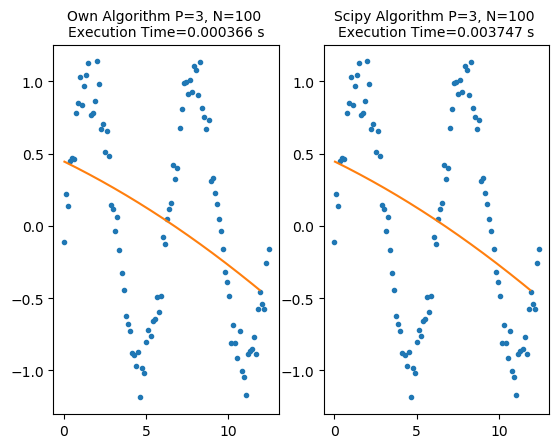
\includegraphics[width=0.5\linewidth,height=0.3\linewidth]{comparison-P=3,N=100.png} &   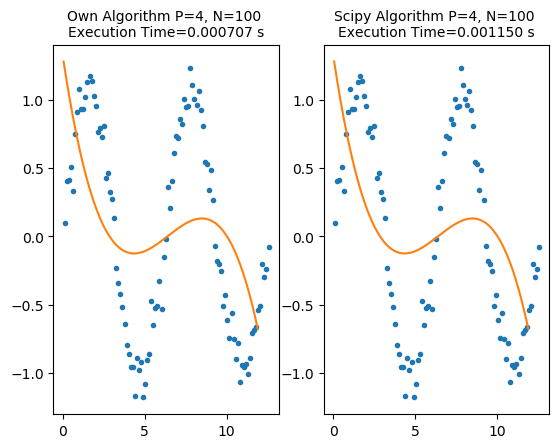
\includegraphics[width=0.5\linewidth,height=0.3\linewidth]{comparison-P=4,N=100.png} \\
  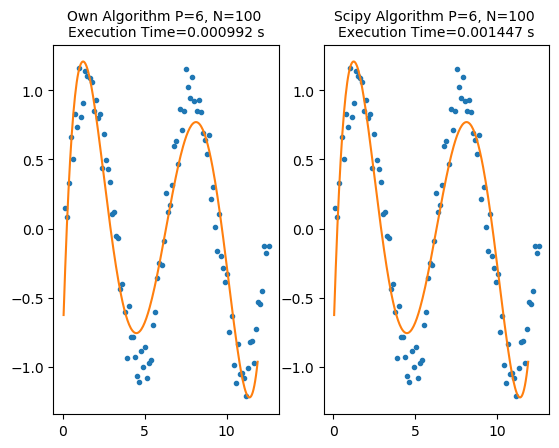
\includegraphics[width=0.5\linewidth,height=0.3\linewidth]{comparison-P=6,N=100.png} &   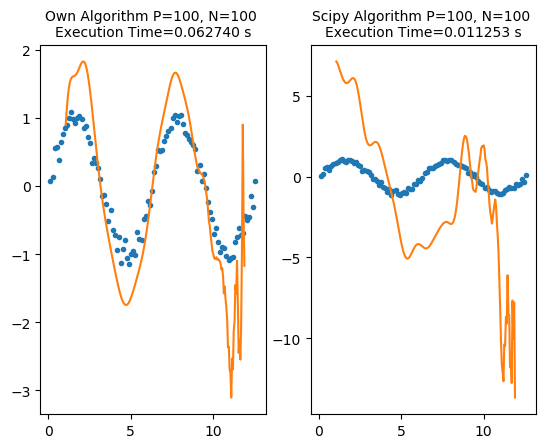
\includegraphics[width=0.5\linewidth,height=0.3\linewidth]{comparison-P=100,N=100.png} \\
\end{tabular}
\end{figure}

\begin{figure}
\begin{tabular}{cc}
  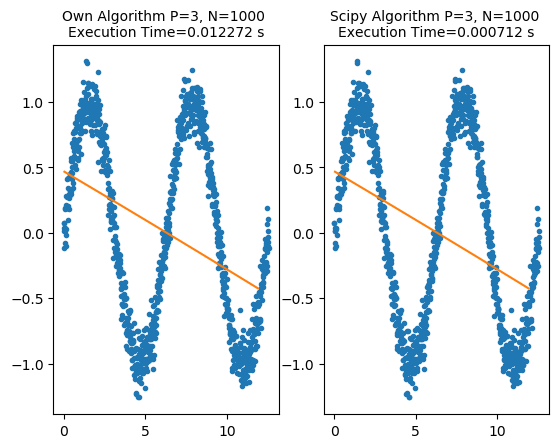
\includegraphics[width=0.5\linewidth,height=0.3\linewidth]{comparison-P=3,N=1000.png} &   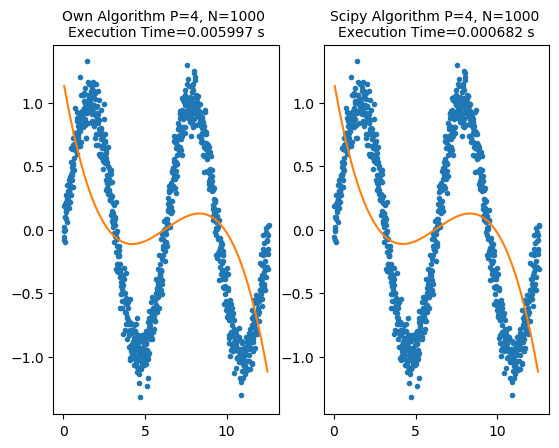
\includegraphics[width=0.5\linewidth,height=0.3\linewidth]{comparison-P=4,N=1000.png} \\
  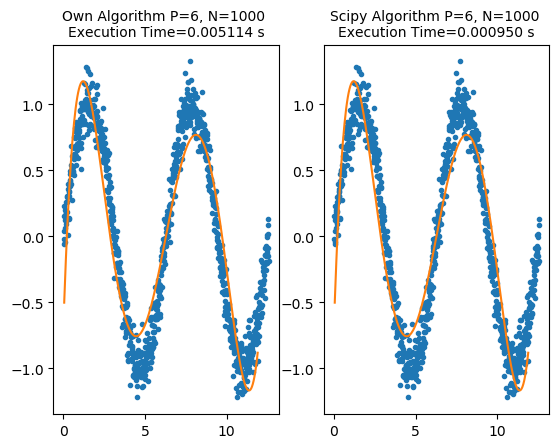
\includegraphics[width=0.5\linewidth,height=0.3\linewidth]{comparison-P=6,N=1000.png} &   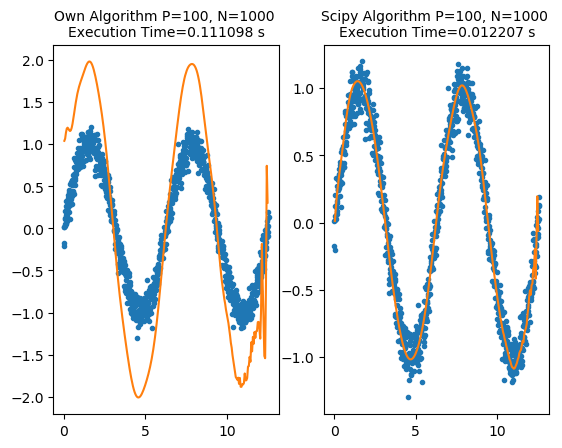
\includegraphics[width=0.5\linewidth,height=0.3\linewidth]{comparison-P=100,N=1000.png} \\
\end{tabular}
\end{figure}

\begin{figure}
\begin{tabular}{cc}
  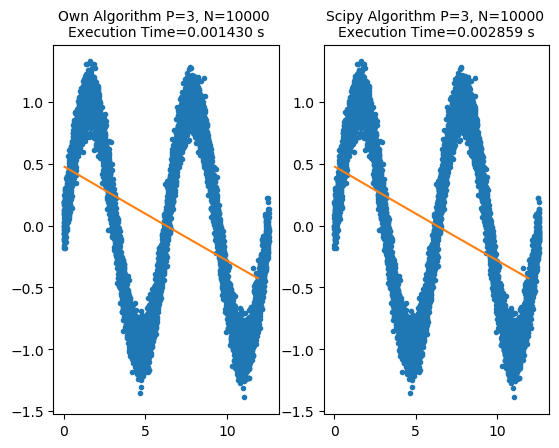
\includegraphics[width=0.5\linewidth,height=0.3\linewidth]{comparison-P=3,N=10000.png} &   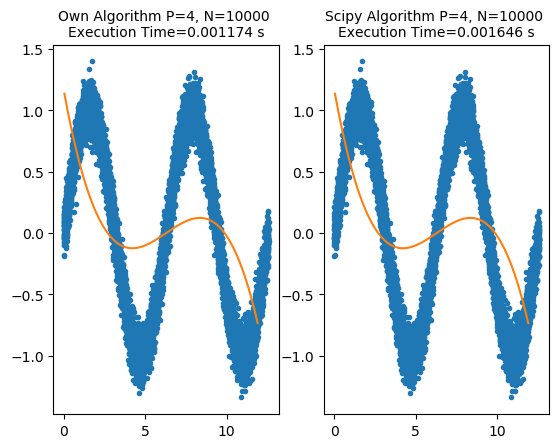
\includegraphics[width=0.5\linewidth,height=0.3\linewidth]{comparison-P=4,N=10000.png} \\
  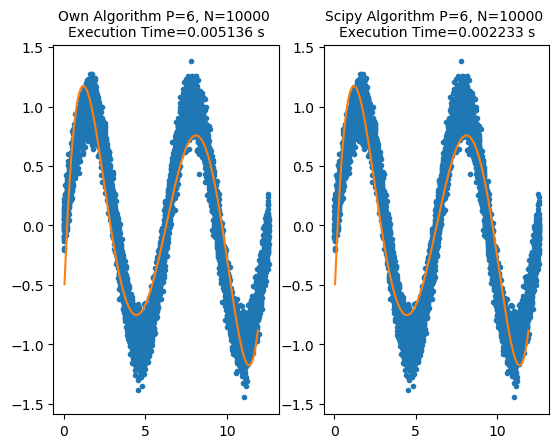
\includegraphics[width=0.5\linewidth,height=0.3\linewidth]{comparison-P=6,N=10000.png} &   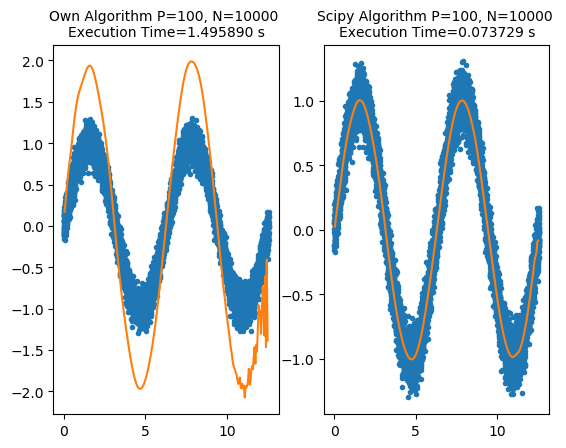
\includegraphics[width=0.5\linewidth,height=0.3\linewidth]{comparison-P=100,N=10000.png} \\
\end{tabular}
\end{figure}

\textbf{Nota} : Es interesante comparar el ajuste obtenido entre nuestro algoritmo implementando el proceso de Gram-Schmidt modificado y la descomposici\'on \textbf{QR} obtenida con la libreria \textbf{scipy}. Es claro notar la diferencia en el ajuste en los casos $P=100, N=1000$ y $P=100, N=10000$. Esta diferencia surge ya que el proceso de \textit{Gram-Schmidt Modificado} sufre de algunos problemas de estabilidad (mucho que menos que el proceso clasico) y en la librer\'ia \textbf{scipy} se implementa una versi\'on optimizada del algoritmo que utiliza reflecciones de Householder \cite{scipy} que es numericamente un poco m\'as estable \cite{wikipediapage}. \\

Otra cosa que se debe mencionar es el caso $P=100, N=100$ que claramente presenta un ajuste muy malo a los datos generados. Esto se debe a que al considerar la soluci\'on de m\'inimos cuadrados esperamos que trabajar con un sistema sobredeterminado, cuando tenemos muchos m\'as datos ( el n\'umero de ecuaciones, N ) que el grado del polinomio a ajustar ( el n\'umero de incognitas, P ). Procuramos graficar el polinomio en el rango $(1, 12)$ para evitar que en el eje de graficaci\'on $y$ el polinomio se salga de un rango considerable e.g $(-3,3)$ y podamos ver un poco m\'as a detalle el ajuste. \\

En la figura~\ref{fig:polinomialFitN=10000} graficamos los ajustes polinomiales con el mismo tama\~no de muestra para diferentes grados del polinomio.

\begin{figure}[!h]
\centering
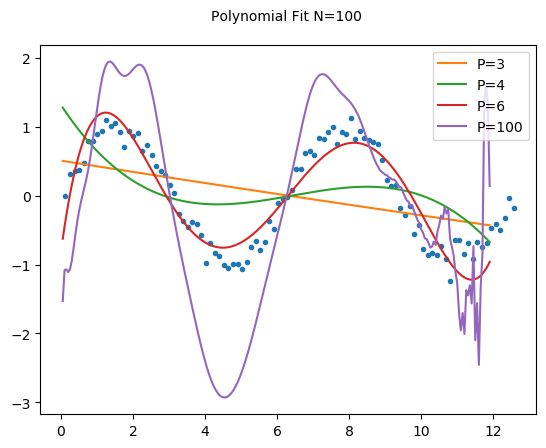
\includegraphics[width=0.6\linewidth,height=0.38\linewidth]{polynomial-fit-N=100.png}
\label{fig:polinomialFitN=100}
\end{figure}

\begin{figure}[!h]
\centering
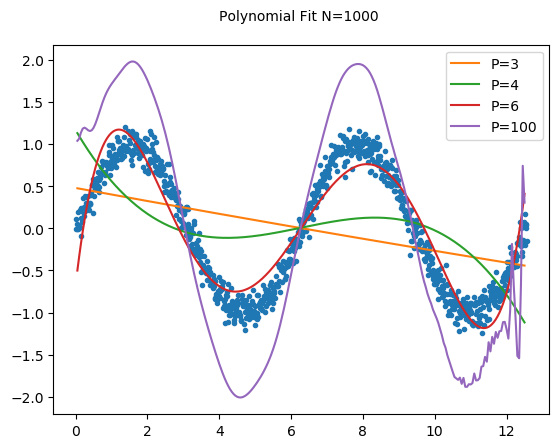
\includegraphics[width=0.6\linewidth,height=0.38\linewidth]{polynomial-fit-N=1000.png}
\label{fig:polinomialFitN=1000}
\end{figure}

\begin{figure}[!h]
\centering
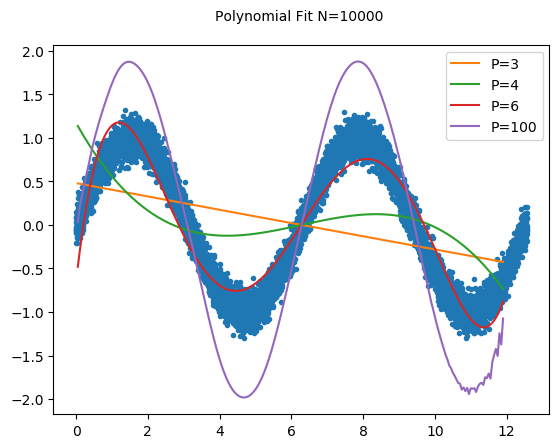
\includegraphics[width=0.6\linewidth,height=0.38\linewidth]{polynomial-fit-N=10000.png}
\caption{}
\label{fig:polinomialFitN=10000}
\end{figure}

En la figura~\ref{executiontimecomparison} gr\'aficamos los tiempos de ejecuci\'on ( medido con \textbf{timeit} ) de todo el algoritmo (no solo la factorizaci\'on QR) que ajusta un polinomio de grado $p - 1$  usando m\'inimos cuadrados. Hacemos la comparaci\'on entre le algoritmo que usa nuestra implementaci\'on de la factorizaci\'on \textit{QR} con el que utiliza el modulo de \textbf{scipy} para calcularla.

\begin{figure}[!h]
\centering
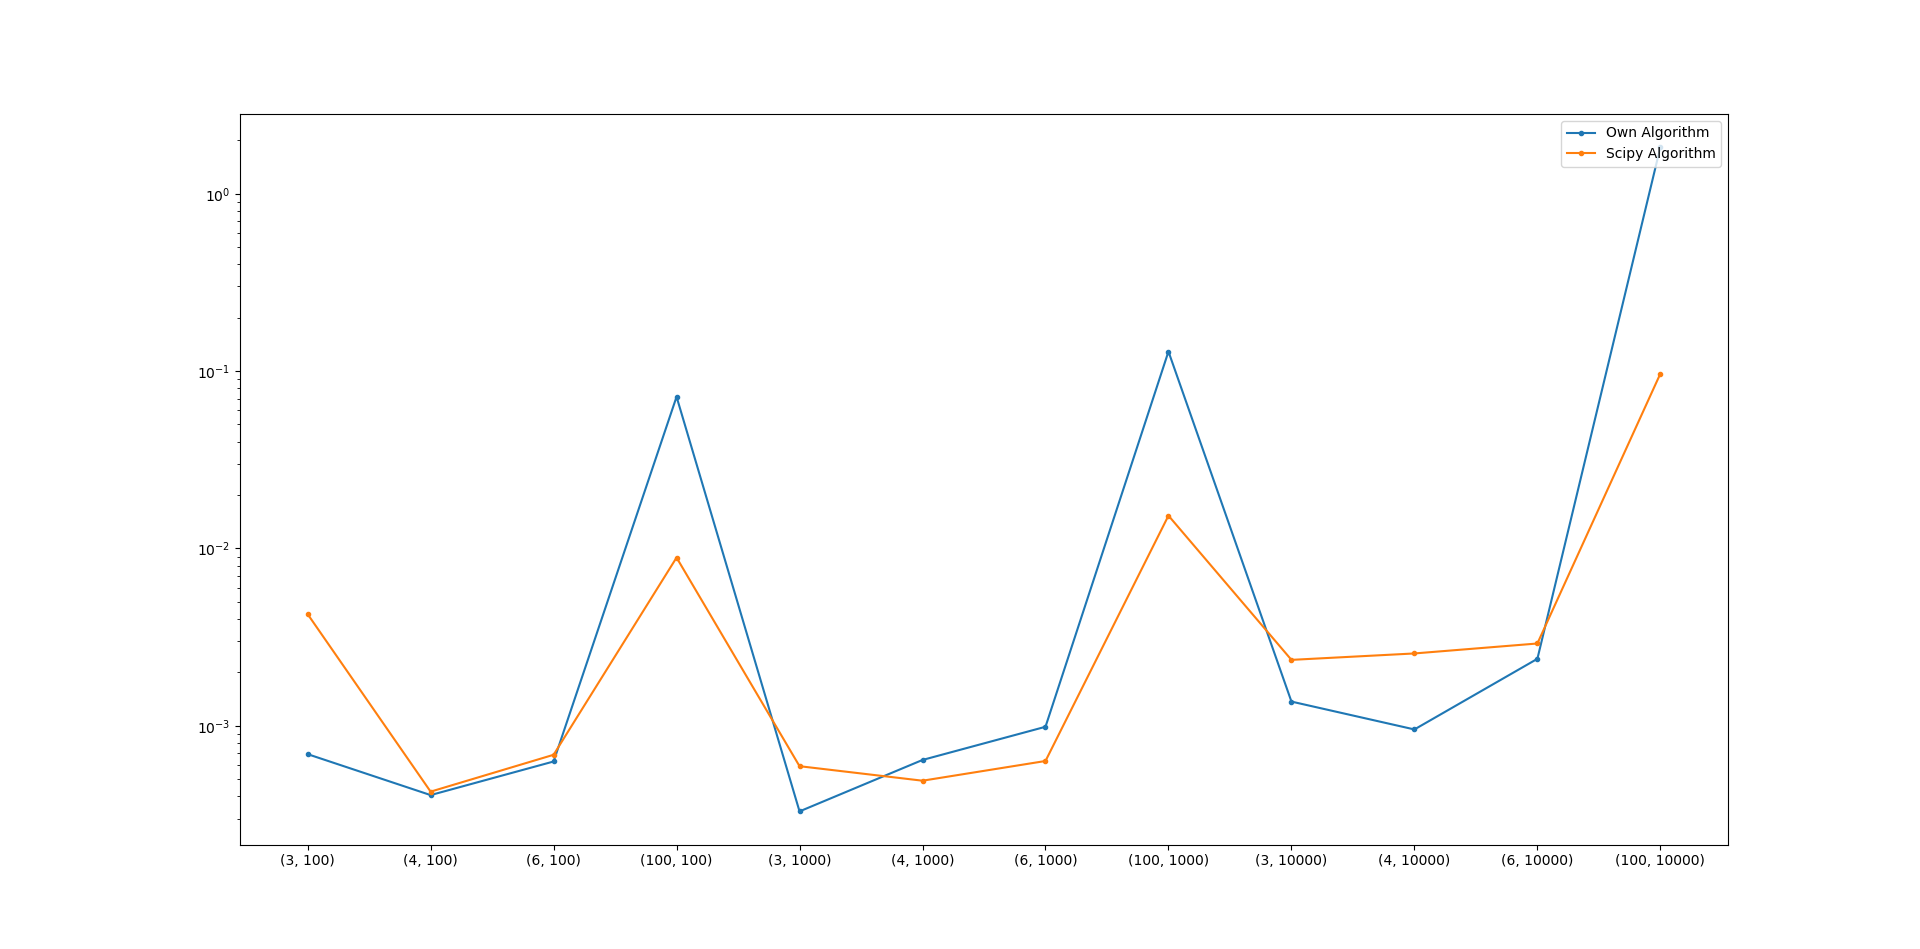
\includegraphics[width=0.8\linewidth,height=0.5\linewidth]{execution-times.png}
\caption{Comparaci\'on de los tiempos de ejecuci\'n (en escala logaritmica) de los 12 casos de la forma (P, N).}
\label{executiontimecomparison}
\end{figure}

\section*{Problema 4}
\textbf{Hacer p = 0.1n, o sea, diez veces m\'as observaciones que coeficientes en la regresi\'on, \textquestiondown Cu\'al es la m\'axima que puede manejar su computadora? }

El m\'aximo valor que la computadora puede manejar es $N = 2810$, osea que $P = 281$. Esto se debe a que al calcular la matriz de Vandermonde ocurre un overflow en la representaci\'on en punto de flotante cuando tenemos que calcular los elementos de las \'ultimas columnas e.g. $x_1^{p-1},  x_2^{p-1}, x_3^{p-1}, ..., x_n^{p-1}$, pues se vuelven productos entre valores muy peque\~nos o muy grandes. \\

El archivo de python \textbf{compare.py} contiene la implementaci\'on de todas las comparaciones y gr\'aficas de esta tarea. Ejecutandolo podemos verficar que es posible manejar el caso $N=2810$ y ver su ajuste. En el primer caso que se encontr\'o un overflow fue cuando $N=2820$, mencionado como warning de python.

En la figura~\ref{executiontimecomparison1} vemos el tiempo de ejecuci\'on de los ajustes con \textbf{p = 0.1n}. 

\begin{figure}[!h]
\centering
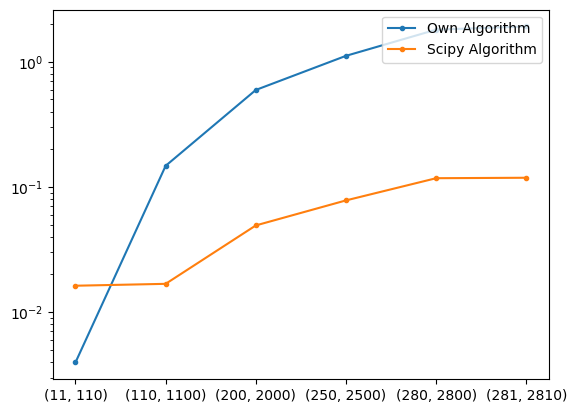
\includegraphics[width=0.8\linewidth,height=0.5\linewidth]{execution-times-6.png}
\caption{Comparaci\'on de los tiempos de ejecuci\'on de casos de la forma (P, N).}
\label{executiontimecomparison1}
\end{figure}

\begin{thebibliography}{9}

\bibitem{scipy} 
scipy.linalg.qr, numpy.linalg.qr, Scipy Documentation
\\\texttt{https://docs.scipy.org/doc/scipy-0.16.1/reference/generated/scipy.linalg.qr.html}
\\\texttt{https://docs.scipy.org/doc/numpy-1.12.0/reference/generated/numpy.linalg.qr.html}


\bibitem{wikipediapage} 
QR decomposition, Wikipedia
\\\texttt{https://en.wikipedia.org/wiki/QR\_decomposition}

\end{thebibliography}

\end{document}
